%!TEX root = ../these.tex

\section{Численные эксперименты}
\label{sec:ccp.exp}

Результаты экспериментов см. в Табл.~\ref{tab:ccp-vs-gtsp}\dots

\begin{table}[b]
  \centering
  \caption{Сравнение качества решений задач CCP и GTSP}
  \label{tab:ccp-vs-gtsp}
  \def\arraystretch{1.2}
  \begin{tabular}{l|*{4}{r}}
      Задание & № 229 & № 464 & № 3211 & № 20205 \\
      \hline
      Кол-во деталей & 11 & 14 & 17 & 115 \\
      Кол-во контуров & 12 & 21 & 22 & 198 \\
      Общий периметр, м & 24.609 & 21.717 & 25.051 & 143.467 \\
      Кол-во точек GTSP & 491 & 429 & 493 & 3917 \\
      $\mathcal L_{GTSP}$, м & 7.729 & 4.743 & 4.557 & 26.098 \\
      $\mathcal L_{CCP}$, м & 7.727 & 4.706 & 4.536  & 25.987 \\
      См. & Рис. \ref{fig:ccp-229} & Рис. \ref{fig:ccp-464} & Рис. \ref{fig:ccp-3211} & Рис. \ref{fig:ccp-20205} \\
      \hline
  \end{tabular}
\end{table}

\makeatletter
  \@for\job:={229,464,3211}\do{
    \begin{figure}
      \centering
      \subfloat[Точное решение задачи GTSP]{
        \includegraphics[width=0.95\textwidth]{\job-gtsp.png}
      }
      \\
      \subfloat[Решение задачи CCP]{
        \includegraphics[width=0.95\textwidth]{\job-ccp.png}
      }
      \caption{Решения задач резки для задания № \job}
      \label{fig:ccp-\job}
    \end{figure}
  }
\makeatother

\begin{figure}
  \centering
  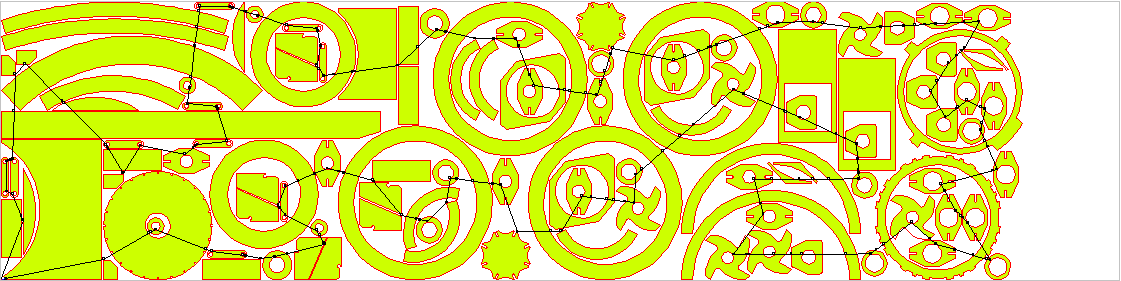
\includegraphics[angle=90,height=0.85\textheight]{20205-ccp.png}
  \caption{Пример решения задачи CCP большого размера, задание № 20205}
  \label{fig:ccp-20205}
\end{figure}
